\subsection{Image Analysis}
	\gls{ia} is the use of various techniques such as pattern recognition, 
	geometry calculations, and signal processing to extract information from 
	digital images for later use. Image processing however is the application 
	of various processes on an image to change or improve the way it looks. The 
	processing stage normally comes before the analysis stage in an effort to 
	simplify the analysis processes and improve their success.
	\subsubsection{Digital Camera Operation}
	A digital camera operates by capturing visible light reflected by objects 
	onto the camera's sensor. The light must travel from the object through a convex focusing lens 
	which refracts the light onto a suitable point on the sensor.
	\begin{figure}[h!]
		\centering
		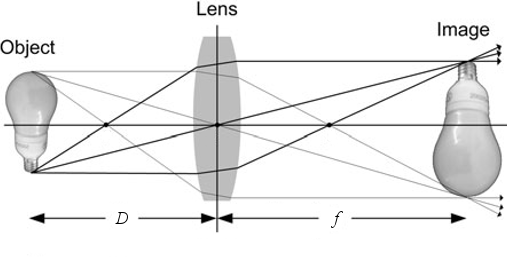
\includegraphics[width=10cm]{../images/camera_bulb.PNG}
		\caption{Diagram of camera and lens operation \citep{introtoprocessing}}
		\label{fig:camera_diagram}
	\end{figure}
	\\\\
	The distance between where light enters the lens and the point at which it is no longer 
	diffused is known as the focal length, marked $f$ in figure \ref{fig:camera_diagram}. This 
	point can be adjusted by changing the lens optics so that the refracted 
	light hits the sensor creating an in focus image.
	\\\\
	A camera's sensor is made up of an array of photosensitive cells capable of collecting light and generating an integer value based on the brightness and colour of the received light. The microprocessor inside the camera takes these values and converts them into the image data, sometimes taking an average of the surrounding values to better understand the light which was captured. Each of the individual sensor cells equates to one pixel on the image produced, for 
	example if a camera produces a 1920x1080 image, the sensor has 1920 cells across by 1080 down, otherwise known as a 2 mega-pixel sensor. The larger the sensor in physical size, the more cells it can contain so the better quality images it can produce.
	\\\\
	These integer values in the image data can be manipulated to change the 
	visual image or the values themselves analysed or compared to neighbouring 
	cells in order to locate objects. The processes are known as image processing and image analysis.
	\subsubsection{Lighting Conditions}
	When capturing images to be analysed, it is important that the lighting conditions are correct so features are not lost \citep{introtoprocessing}. If the image is captured in unsuitable conditions then this can seriously affect the outcome of any analysis techniques applied. Some image processing techniques can fix bad lighting conditions though this can prove difficult. The effects of different lighting angles can be seen in figure \ref{fig:illumination}.
	\begin{figure}[h!]
		\centering
		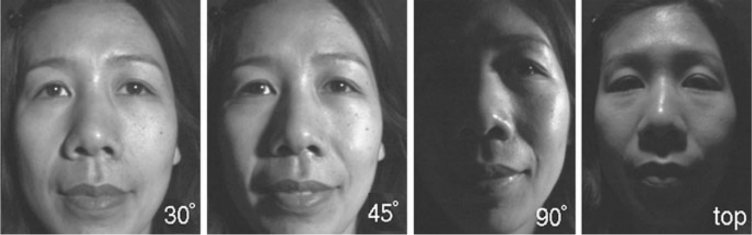
\includegraphics[width=\linewidth]{../images/face_illumination.png}
		\caption[]{The effects of different lighting conditions on a face \citep{introtoprocessing}}
		\label{fig:illumination}
	\end{figure}\\
	It can be seen that the situation which highlights the most features is direct illumination; this reduces the amount of image processing required before analysing. Many cameras have a built in flash which can be used to correctly light the subject of the image and in the context of this project many smartphones also have a flash function. This solves the need for the user to correctly light their image capture as the flash can be applied automatically if needed.
	\subsubsection{Usages}
	Image processing and analysis has been applied to multiple areas with its value and 
	effectiveness rapidly improving alongside camera technology and computing power. These 
	applications range from recognising faces in social media uploads \citep{zuckerberg2011tagging} 
	to the utilisation of satellite imagery for tracking the changing shape of coastlines 
	\citep{costalimagery}.
	\begin{figure}[h!]
		\centering
		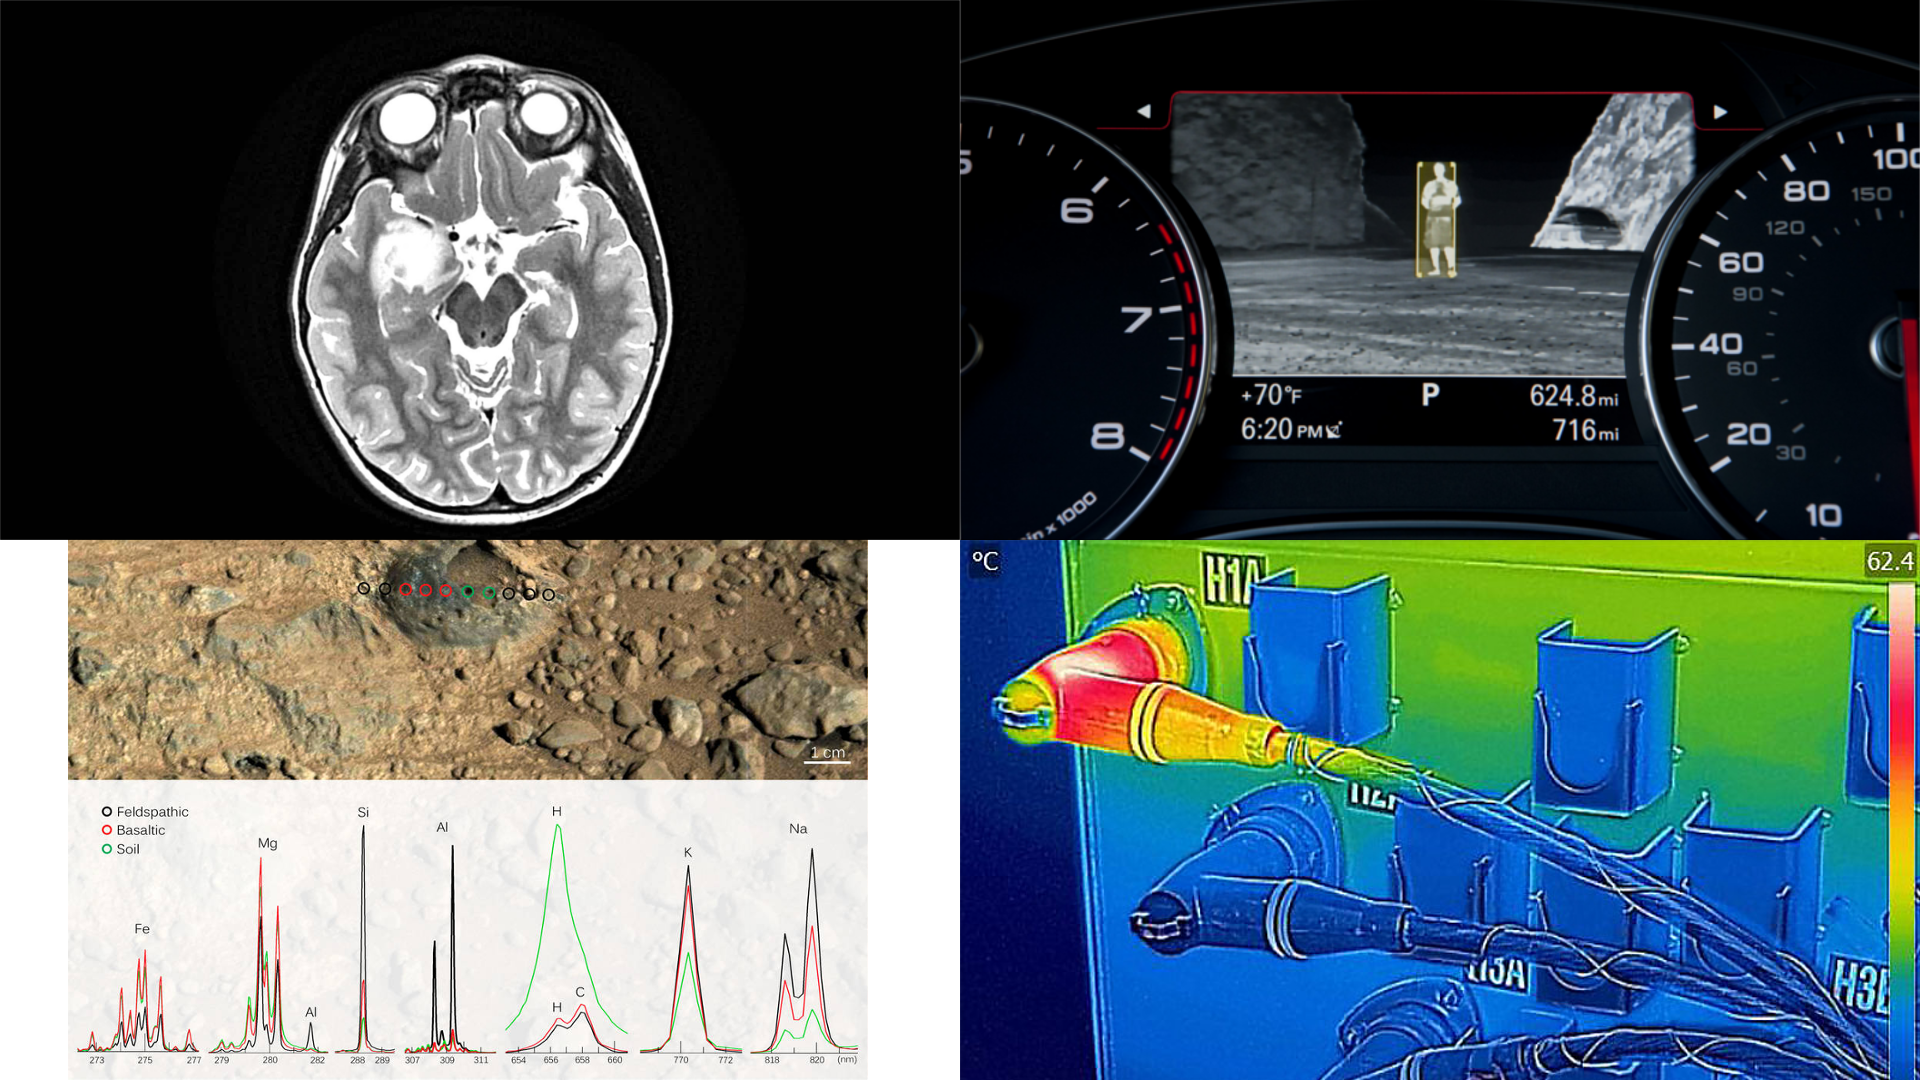
\includegraphics[width=15cm]{../images/4panel.png}
		\caption[Uses of image analysis]{Uses of image analysis, from top left clockwise: An MRI brain scan, automotive 
		night vision with pedestrian recognition, infrared image taken with a smartphone, chemical 
		rock analysis from 
			mars}
		\label{fig:analysis_uses}
	\end{figure}
	\paragraph{Medical}
	Arguably one of the most important uses of \gls{ia}, advances in medical imaging have reduced costs, diagnosis time, recovery time, and improved the ability to localise and personalise treatments \citep{esfmedical}. Major uses of \gls{ia} in medical applications are Magnetic Resonance Imaging (MRI) and Computerised Topography Scanning (CT Scan) to create detailed images of the human body and identify illness before most symptoms arise. This is shown top left in Figure \ref{fig:analysis_uses}.
	\paragraph{Transport}
	Image analysis has been included in the consumer automotive market on various models since 2004 when Honda introduced an thermographic night vision camera with pedestrian detection on the Legend  \citep{hondanightvision}, Audi's implementation can be seen top right in figure \ref{fig:analysis_uses}. Since this initial introduction many vehicle manufacturers have included image analysis and recognition features as options such as speed limit sign recognition, lane departure warning systems, and automatic braking systems based on hazard recognition.
	\paragraph{Engineering}
	The use of image analysis in engineering has pushed to create more stable and efficient structures by looking at the materials used in their construction \citep{concreteanalysis} and monitoring their stresses and potential weak areas \citep{bridgecables}. Using image analysis by engineers on site has become more common with the advances in mobile computing and some manufacturers aiming their products at an engineering demographic with features like improved durability and built in infrared imaging \citep{catphone}, the output of which can be seen lower right in figure \ref{fig:analysis_uses}.
	\paragraph{Space}
	While some industries make use of satellite imagery to monitor changes on our own planet, agencies such as NASA and ESA make use of image analysis to look at other planets and celestial bodies. The Martian rover, Curiosity, uses multiple cameras for navigation, hazard avoidance, and scientific imaging the products of which are streamed back to Earth for analysis. Major uses for the various types of images returned include identification of geological formations and compositions \citep{curiositysand, curiositygravel} and chemical location and identification using the "ChemCam" \citep{curiosityhydrogen}. Chem cam analysis can be seen lower left in figure \ref{fig:analysis_uses}.